\chapter{Performance énergétique théorique et réelle}

........La méthode de suivi et d'évaluation innovante du CEREMA doit être évoquée: % Pôle R&D\Thèse_Cifre\Admin_Quentin\Conférences et réunions\Evenements Paris\Colloque Rexbatex (derniere page) 

Nous venons d'évoquer le contexte global de la conception et de la construction sous l'angle d'un bureau d'études thermique et environnement. Le travail de ce type de structure est de donner un avis d'expert sur les questions énergétiques. Pour cela, les outils numériques comme les Simulations Thermiques Dynamiques (STD) sont utilisés afin de modéliser les futures constructions et donc prédire leurs performances.

Or des doutes émanent sur la fidélité des modèles à reproduire les phénomènes énergétiques des bâtiments. Cette différence entre ce qui est prédit et ce qui est mesuré n'est généralement pas anecdotique et portent le nom \textit{performance gap}. Les performances des bâtiments sont influencées par de nombreux facteurs, tels que les conditions climatiques, les équipements et la structure du bâtiment, mais aussi à des facteurs relatifs aux occupants eux mêmes, comme leurs comportements, leurs conditions environnementales intérieures et la maintenance de leurs équipements. Les effets de la modélisation du climat, de l'enveloppe et des systèmes sont bien connus et standardisés, alors que ceux en lien à l'utilisation du bâtiment se révèlent être plus incertains. On comprend alors que prédire les consommations totales des bâtiments est un exercice très complexe si l'on considère tous ces éléments.

Cela doit néanmoins être réalisé pour quantifier et garantir les performances des travaux de rénovation mais aussi de construction. Cette garantie devient alors une sécurité pour les donneurs d'ordres qui peuvent évaluer les risques de rénover un bâtiment ou de rechercher une performance énergétique d'excellence. Parce que le travail de donneur d'ordres est un travail à risque, la contractualisation de garantie énergétique peut permettre de sécuriser les opérations incertaines. Ce travail de Contrat de Performance Énergétique (CPE) est traité dans ce chapitre de l'angle juridique, financier, technique mais aussi et surtout vu de l'angle méthodologique. Ce chapitre est donc l'occasion de présenter ce qu'est le \textit{performance gap}, de présenter les raisons en phase de conception, chantier, exploitation et maintenance et donc de terminer sur la contractualisation d'une assurance de performance.

\section{Le \textit{performance gap}}
\label{performance gap}

Améliorer les performances énergétiques et le confort des bâtiments est un objectif indispensable mais aussi très général. Dans l'esprit du plus grand nombre, ces améliorations passent par un meilleur bioclimatisme et des systèmes plus performants. Or, mieux prédire ce qui est envisagé et mieux vérifier se qui se passe réellement permet également de gagner en qualité, ainsi qu'une optimisation continue des processus de conception, de construction et d'exploitation.

Une mise à jour des outils de prédictions actuels est alors nécessaire afin de mieux considérer les paramètres d'influences. Plusieurs groupes de recherche revoient les hypothèses pour les prévisions de performances énergétiques des bâtiments et de confort. L'Agence Nationale de la Recherche (ANR) "Fiabilité des prévisions des performances énergétiques des bâtiments" \footnote{http://www.agence-nationale-recherche.fr/?Projet=ANR-10-HABI-0004} se positionne dans la garantie de performance énergétique par une revue de l'usage des outils de STD. Le projet Tribute\footnote{http://www.tipee-project.com/projets/le-projet-tribute} souhaite quant à lui revoir tous les paramètres influents les performances, y compris le vieillissement des matériaux.

Entre 1975, date de la première réglementation thermique, et les années 1990, les bâtiments étaient construits en suivant des exigences de moyens et non pas de résultats. L'atteinte de performance minimum n'était alors pas la préoccupation première de la maîtrise d'ouvrage. Avec le développement des premiers outils numériques de prédiction des consommations énergétiques dans les années 1990, il est petit à petit devenu possible de fixer des exigences de résultats plutôt que de moyens. En 1994, Norford et al. \cite{Norford-94} de l'Université de Princeton ont été les premiers à mettre en avant les différences entre les modèles et les résultats sur un bâtiment de bureau modélisé sous le logiciel DOE-2. A cette époque les efforts étaient menés sur la modélisation des systèmes de Chauffage, Ventilation et Climatisation (CVC), alors que la modélisation du bâti était déjà assez fiable pour les matériaux courant. Plus tard, les chercheurs sont parvenus à prendre en considération les phénomènes dynamiques et notamment les apports solaires et sollicitations extérieures. En revanche, l'attention n'était pas spécialement portée sur les actions des occupants car celles-ci avaient un impact plus faible. En effet, ces actions sont devenues plus impactantes énergétiquement suite aux progrès réalisés sur le bâti. De même, si l'on raisonne en relatif, la prise en compte du vieillissement des systèmes et des matériaux est plus significative pour des constructions performantes. 

Depuis plusieurs dizaines d'années il est facile de trouver des études qui quantifient les écarts entre les consommations théoriques et réelles des bâtiments. Une plateforme collaborative, CarbonBuzz \footnote{Site internet \url{http://www.carbonbuzz.org/}}, a d'ailleurs été lancée pour recenser les \textit{performances gap} des bâtiments. Les résultats montrent généralement des écarts très significatifs, avec des consommations réelles pouvant excéder de 250\% les consommations estimées et une moyenne de dépassement comprise entre 150\% et 200\%. Ces retours d'expériences montrent que les outils informatiques n'ont pas suivi les améliorations continues de la performance énergétique des bâtiments mais qu'il existe tout de même une marge de progression pour cette modélisation.

Nous venons de voir que les logiciels actuels de STD sont perfectibles, néanmoins ces outils ayant vocation à être utilisés dans l'industrie il est essentiel de considérer le coût de ces efforts. Cette démarche de qualité de la modélisation doit également être menée dans une logique de recherche d'optimum entre un niveau raisonnable d'incertitude du modèle et un coût maitrisé. En effet le coût de la sur-perfection peut se révélé plus élevé que le coût de la non-qualité. L'outil idéal pour les bureaux d'études est fiable techniquement mais également simple et rapide à utiliser.

\section{Conception}

Une des causes du \textit{performance gap} peut être attribué à l'énergéticien qui a réalisé l'étude. En effet, réaliser une bonne STD dépend énormément des connaissances que le modélisateur a du bâtiment ainsi que de son usage. Plus le nombre d'hypothèses qu'il fait est élevé plus l'estimation sera incertaine. La communication entre les différents acteurs de la conception est alors une des clés pour réduire les écarts entre performance théorique et réelle. En effet, si la maîtrise d'ouvrage communique fréquemment avec la maîtrise d'œuvre et lui permet de définir fidèlement l'intensité d'usage et les scénarios d'occupations alors la qualité de la prédiction ne pourra en être que meilleure. Aussi, le niveau de maturité du projet influence la finesse des résultats, les résultats d'un projet en phase d'études d'Avant-Projet Sommaire (APS) sont évidement bien plus incertains qu'en phase PROjet (PRO). 

Nous pouvons en profiter pour noter ici que l'influence du simulateur pour une étude réglementaire est beaucoup plus faible qu'en STD, car les paramètres d'entrées sont moins nombreux et les scénarios d'utilisation sont définis par la règlementation. Réaliser un calcul RT peut alors être vu comme réaliser une étude STD bridée par la règlementation en vigueur. De plus, en aucun cas les études règlementaires doivent être utilisées pour prédire des performances ou consommations, ces études servent uniquement à vérifier qu'un bâtiment est conforme à la réglementation.

Par nature les logiciels de modélisation n'ont pas les mêmes propriétés les uns des autres, le choix du logiciel a donc une influence directe sur les résultats. Al-Koussa \cite{AlKoussa-14} propose une comparaison qualitative des comportements et résultats des logiciels Dymola, Simulink, ESP-r et TRNSYS. Réaliser deux simulations identiques sur deux logiciels différents, ne mène donc pas à deux résultats exactement identiques.

Ainsi, pour réduire le \textit{performance gap}, l'énergéticien doit bien connaître les forces et faiblesses de ses outils pour utiliser celui qui est le plus approprié à son projet. Il doit également en fonction de l'avancement du projet adapter le niveau de finesse de son modèle. Cela passe par une communication étroite avec la maîtrise d'ouvrage qui doit se tenir à sa disposition afin de minimiser le nombre d'hypothèses et d'incertitudes. Enfin, le travail du simulateur doit être rigoureux pour être en mesure de revenir sur des hypothèses finalement levées et ainsi réduire le tunnel d'erreur de la simulation.

\section{Construction}

Nous venons de voir que la qualité des études de conception dépend beaucoup des connaissances de l'énergéticien sur le projet et du logiciel utilisé. Néanmoins, ces études ne prennent pas en compte des éventuels défauts de construction, or la qualité du chantier doit également être remise en question dans le cadre de la maîtrise des performances énergétiques. En effet, en phase de construction il est nécessaire d'être vigilant sur la mise en place des différents éléments. 

Les professionnels du secteur ont parfois peu de formation sur la mise en œuvre de techniques performantes d'un point de vue énergétique. Les bâtiments performants font appel à des techniques constructives nouvelles, qui ne sont pas toujours parfaitement maîtrisées par les entreprises du bâtiment. Parmi les défauts de construction constatés, il est fréquent d'observer des discontinuités d'isolant, des infiltrations d'air au niveau du réseau électrique et fluide, des pares-vapeur mal installés ou encore des joints d'étanchéité mal posés sur les menuiseries. Cette liste non-exhaustives de défauts de construction est résultante de professionnels pas toujours qualifiés ou appliqués, de désaccords entre les artisans des différents corps d'état ou encore d'une supervision des travaux insuffisante. Ces raisons qui peuvent expliquer une mauvaise qualité du chantier sont à encadrer pour éviter des dérives des consommations. En effet, le suivi continu des étapes du chantier évite que la non-qualité ne se généralise dans le bâtiment. 

Pour encadrer l'évaluation de la qualité sur les chantiers et donc répondre aux besoins des conducteurs de travaux et aux maîtres d'œuvre, des logiciels rendent possible un contrôle qualité des ouvrages. Ces logiciels disponibles sur tablettes numériques et smart-phones facilitent l'identification des problèmes de qualité tout au long du chantier. Ces applications, telles que FinalCAD \footnote{Site internet: \url{http://www.finalcad.com/fr/}, visité le 23/12/2015} ou Air-Bat\footnote{Site internet: \url{http://www.air-bat.fr//}, visité le 23/12/2015} permettent donc d'effectuer les relevés de réserves sur le chantier, puis dans un deuxième temps de contrôler, corriger et générer les procès verbaux. Ce suivi numérique rend alors possible un contrôle qualité exhaustif tout au long du chantier sur la totalité des points clés de l'ouvrage.

La qualité chantier est donc un gage de limitation du \textit{performance gap}, c'est à dire de maîtrise des consommations énergétiques et de confort des occupants.

\section{Exploitation}

La parfaite livraison d'un bâtiment n'est pas la certitude, loin de là, d'un faible écart entre performance théorique et réelle. La manière dont l'exploitation est faite par ses usagers, ainsi que les phénomènes météorologique influent sur les performances réelles.

\subsection{Usages et usagers}

Il est confirmé par de nombreux scientifiques, Hoes \cite{Hoes-09}, Kashif \cite{Kashif-13}, Chen \cite{Chen-12}, que le comportement des usagers est un des paramètres d'entrée influençant le plus les simulations énergétiques des bâtiments. DeMeester et al. \cite{deMeester-13} précisent que le comportement impacte particulièrement les consommations relatives dans le cadre de bâtiments fortement isolés. Il est important de nuancer en précisant qu'en valeur absolue, les différences de consommations entre des comportement vertueux et energivores, dans des bâtiments peu performants restent plus importantes que dans des bâtiments performants. En d'autres mots, l'impact environnemental d'un mauvais comportement dans un bâtiment performant est moins fort que dans une passoire énergétique contrairement à la réduction relative des consommations. Degelman \cite{Degelman-99} confirme lui que les simulations énergétiques sont depuis quelques années proches de la perfection, mais cela uniquement si les bâtiments sont utilisés de manière routinière et prévisible, ce qui n'est jamais le cas. Des études de sensibilité sur l'impact du comportement des occupants, tel que l'état de l'art de Larsen et al. \cite{Larsen-10}, attestent de la nécessité d'être rigoureux dans la modélisation des comportements vis à vis de l'énergie. Dans ce document technique, 1000 logements similaires ont été suivis dans la banlieue de Copenhague et après pondération des résultats, les consommations finales d'énergie montrent d'énormes différences dues aux pratiques des occupants. 

Toutes ces études montrent finalement qu'en fonction des usages et usagers, un bâtiment performant peut consommer davantage qu'un bâtiment théoriquement moins performant. Dans les deux sections suivantes, nous proposons de reprendre la définition du comportement des occupants de Zaraket \cite{Zaraket-14} qui distingue une part rationnelle du comportement d'une autre aléatoire.

\subsubsection{Rationalité}

Dans le contexte du bâtiment, et principalement en résidentiel, les actions des occupants impactant les consommations énergétiques sont nombreuses, tout comme les paramètres influant le comportement des occupants vis à vis de l'énergie. Cette complexe relation entre les occupants et leur environnement est présenté schématiquement dans la Figure \ref{fig:Comportement_occupant_energie}. Ce schéma traduit en français à partir des travaux de l'Annexe 53 \cite{Annex-53-1} de l'Agence Internationale de l'Énergie (IEA), présente et organise l'ensemble des paramètres modifiant les comportements humains vis à vis de l'énergie. On note deux grands types de paramètres influant ces comportements, d'un coté les paramètres internes (biologique, psychologique et social) qui concernent directement les occupants et de l'autre les paramètres liés aux bâtiments et aux conditions environnementales. Les paragraphes suivants détaillent en quoi le genre, les interactions de groupe et la facilité de l'opération modifient les consommations énergétiques.

\begin{figure}[h]
\centering
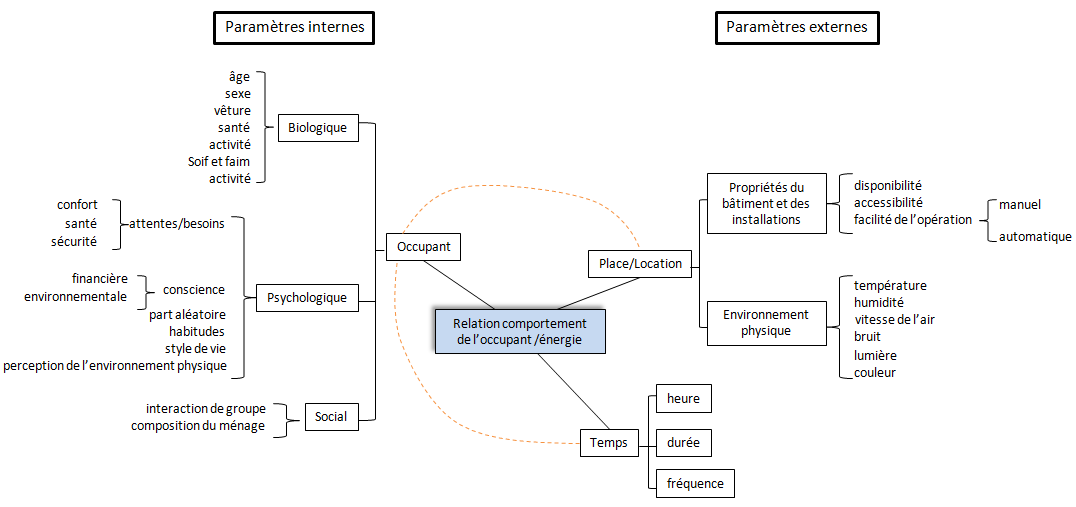
\includegraphics[scale=0.6]{Images/Comportement_occupant_energie}
\caption{Relation entre le comportement des occupants et les consommations d'énergie}
\label{fig:Comportement_occupant_energie}
\end{figure}

\paragraph{Genre}

La Figure \ref{fig:Comportement_occupant_energie} indique que le sexe est un paramètre biologique qui influe sur les consommations énergétiques. En effet, plusieurs études physiologiques ont montré que les femmes et les hommes n'ont pas les mêmes attentes en terme de confort. En effet, Foda et al. \cite{Foda-11} et Jacquot et al. \cite{Jacquot-14} ont montré que les sentions thermales ne sont pas identiques selon le genre, cela modifie donc les températures de consigne et en conséquence les consommations énergétiques. Il a été prouvé que les femmes ont tendance à moins bien supporter le froid que les hommes, alors que ces derniers sont plus vulnérables face aux températures élevées.

\paragraph{Interactions de groupe}

Une communauté scientifique de sociologues de l'énergie se développe afin de mieux comprendre les comportements humains vis à vis de l'énergie et notamment les effets de groupes. Dans ce cadre, des Journées Internationales de la Sociologie de l'Énergie \footnote{Site officiel des deuxièmes JISE 2015 à Tours: \url{http://www.socio-energie2015.fr}} (JISE) s'organisent pour étudier les pratiques courantes des usagers.

Les conflits sur les niveaux de confort dans les bâtiments résidentiels sont fréquents dans tous types de ménages. Les rapports sociaux entre un mari et sa femme, entre des parents sur leurs enfants ou un patron sur ses employés modifient les consommations énergétiques. Certaines relations sont plutôt démocratiques, d'autres sont plus autoritaires, ainsi des règles de priorité peuvent être établies au sein du groupe social. Ainsi, les pratiques liées à l'énergie alimentent un processus de différenciation identitaire entre les membres de la famille: l'un est toujours plus frileux ou économe que l'autre. Aussi, la présence d'invités au domicile est un moment de surconsommation avec des rituels d'accueil (mise en fonctionnement d'appareils de cuisine, augmentation de la température, augmentation de l'intensité lumineuse, musique, etc.) calqués aux normes sociales mais qui participent également à une certaine mise en scène de l'identité familiale.

La définition de règles d'usage et de priorité entre les agents est complexe à définir tant les paramètres d'influence sont nombreux. Alfakara et Croxford \cite{Alfakara-14} dans leurs travaux modélisent les interactions sociales en définissant que l'individu le plus âgé d'une pièce à vivre est celui qui fixera ses conditions de confort ou de volonté, et cela dans un contexte de surchauffe estival. Quelles que soit les règles fixées, il ne faut pas perdre à l'esprit qu'ici l'intérêt est de modéliser les performances et consommations énergétiques plutôt que de modéliser les interactions sociales.

\paragraph{Accessibilité aux systèmes}

Plusieurs études ont montré que lorsque l'on s'intéresse aux actions des occupants dans le bâtiment l'accessibilité aux systèmes de contrôle modifiait les comportements. Sutter et al. \cite{Sutter-06} ont étudié l'utilisation des stores dans les bureaux en fonction de leur accessibilité. Ils en ont conclu que les stores électriques (accessibles à distance) des bureaux étaient trois fois plus utilisés que les stores manuels. Cette étude a été réalisée en observant de l'extérieur le nombre de montées-descentes des stores. 

Andersen \cite{Andersen-09} confirme que l'accessibilité des systèmes de contrôle joue un rôle majeur dans le comportement des usagers et affirme que le temps avant de s'adapter à une zone d'inconfort diminue lorsque les moyens d'adaptation sont nombreux et disponibles. Cette disponibilité des contrôles sur le confort visuel ou thermique modifie alors les comportements adaptatifs des usagers et a en conséquence un impact direct sur le bilan énergétique.

\subsubsection{Aléas}

Nous venons de voir que les comportements humains sont rationnels et qu'ils dépendent de paramètres dits "internes" et "externes". Malgré ces relations plutôt rationnelles entre l'environnement et les actions des occupants, il y a également une part d'insaisissable dans l'humain qui ne réagit pas de manière déterministe à la manière d'un robot. En d'autres mots, un même individu dans un contexte exactement similaire ne réagira pas toujours de la même façon. Les usagers par leurs comportements incertains, rendent les prévisions énergétiques également incertaines. Cette part aléatoire des comportements humains doit ainsi être mieux appréhendée pour l'intégrer aux calculs de performances énergétiques.

Les comportements humains sont donc rationnels et aléatoires. D'après les travaux d'O'Brien et Gunay \cite{O'Brien-14} et de ceux de Leaman \cite{Leaman-99}, les comportements humains sont également parfois surprenants. En effet, ils ont en outre remarqué que certains occupants:
\begin{itemize}
 \item attendent un certain temps avant de s'adapter lorsqu'ils sont en zone d'inconfort
 \item compensent en excès leurs actions à des inconforts mineurs
 \item prennent l'option la plus facile et la plus rapide pour un effet immédiat plutôt que la meilleure 
 \item laissent consciemment ou non les systèmes dans leur état après un changement plutôt que de les réinitialiser après que l'inconfort soit passé
 \end{itemize} 

L'ensemble de ces éléments comportementaux rendent compte de la difficulté d'un exercice de modélisation de l'humain. Néanmoins, la modélisation de ces comportements est une modélisation intermédiaire qui ne sert qu'à améliorer les simulations des bâtiments. Une modélisation fine de l'humain n'apporterait pas spécialement de meilleurs résultats, un optimum de niveau de modélisation est à trouver. En connaissance de cause, nous avons la conviction que modéliser des comportements extrêmement surprenants ou même dérivants, n'améliorerait pas les prédictions énergétiques.

\subsubsection{De la sociologie à l'ingénierie}

Comme nous venons de le voir le comportement des occupants peut se décomposer en une part rationnelle et une part aléatoire. La traduction des études sociologiques en informations exploitables pour des ingénieurs d'études ou de recherche est difficile car les données sont qualitatives plutôt que quantitatives. De plus, ces données sont souvent très disparates et privées de droits. On peut tout de même recenser certains organismes, comme le Centre de Recherche pour l'Etude et l'Observation des Conditions de vie (CREDOC), qui recense quelques données quantitatives sur la façon dont vivent les habitants d'un point de vue social mais également énergétique. 

Dans le but de synthétiser et de catégoriser les paramètres d'influences sur le chauffage, le refroidissement, la ventilation, les opérations sur les fenêtres, l'utilisation de l'eau chaude sanitaire, de l'usage d'électricité et de l'éclairage, l'Annexe 53 \cite{Annex-53-1} a créée des tableaux de synthèse. La Table \ref{tab:drivingforce} présente les niveaux d'importance des paramètres influençant les comportements et la Table \ref{tab:drivingforceheat} est une application pour les comportements vis à vis du chauffage. Le tableau se lit comme: la température de consigne dépend fortement du niveau d'isolation du bâtiment, alors que la durée du chauffage dépend très peu des intentions du gouvernement. L'ensemble des tableaux se trouve dans le rapport final de l'Annexe 53.

\begin{table}[h]
\begin{center}
\begin{tabular}{|c|c|}
\hline
\multicolumn{2}{|c|}{\textbf{Importance}} \\
\hline
\hline Description & Symboles \\
\hline Très hautement significatif ($p\leq 0.001$) & \cellcolor{OliveGreen} *** \\
\hline Hautement significatif ($p\leq 0.01$) & \cellcolor{LimeGreen} ** \\
\hline Modérément significatif ($p\leq 0.05$) & \cellcolor{yellow} * \\
\hline Peu significatif ($p\leq 0.1$) & \cellcolor{orange} ' \\
\hline Pas significatif & \cellcolor{red} p.s. \\
\hline Pas déclaré & \cellcolor{gray} x \\
\hline
\end{tabular}
\caption{Notation utilisée pour l'importance des paramètres influents; la valeur p correspond au niveau statistique}
\label{tab:drivingforce}
\end{center}
\end{table}

\begin{table}[H]
\begin{center}
\small
\begin{tabular}{|p{2cm}||p{2cm}|p{2cm}|p{2cm}|p{1.5cm}|p{2cm}|p{2cm}|}
\hline & Biologique & Psychologique & Sociologique & Temporel & Environnement physique & Bâtiment et équipements \\
\hline
\hline \multirow {3}{1pt}{Consigne de température} & \cellcolor{gray} Genre \cite{Andersen-09} & \cellcolor{yellow} Attentes \cite{Keul-11} & \cellcolor{LimeGreen} Possession (propriétaire, locataire) \cite{Keul-11} & \cellcolor{orange} Heure de la journée \cite{Andersen-09} & \cellcolor{OliveGreen} Température extérieure de l'air \cite{Larsen-10} & \cellcolor{OliveGreen} Niveau d'isolation du bâtiment \cite{Muller-10} \\
\cline{2-7} & \cellcolor{LimeGreen} Habits \cite{Andersen-09}\cite{Keul-11} & \cellcolor{OliveGreen} Fréquence d'interaction avec le système de contrôle \cite{Andersen-09} &  &  & \cellcolor{LimeGreen} Humidité de l'air extérieure \cite{Andersen-09} & \cellcolor{yellow} Type de ventilation \cite{Keul-11} \\
\cline{2-7} &  & \cellcolor{yellow} Ouverture de fenêtre \cite{Andersen-09} &  &  &  &  \\
\hline \multirow {3}{50pt}{Durée de l'activation du chauffage} & \cellcolor{LimeGreen} Habits \cite{Andersen-09}\cite{Keul-11} & \cellcolor{LimeGreen} Compréhension des fonctions de contrôle \cite{Andersen-09}\cite{Keul-11}\cite{Peeters-08} & \cellcolor{Orange} Possession (propriétaire, locataire) \cite{Andersen-09} &  & \cellcolor{OliveGreen} Température extérieure de l'air \cite{Andersen-09} & \cellcolor{OliveGreen} Niveau d'isolation du bâtiment \cite{Muller-10} \\
\cline{2-7} &  &  &  &  & \cellcolor{OliveGreen} Humidité de l'air extérieure \cite{Andersen-09} & \cellcolor{OliveGreen} Type du système de chauffage \cite{Andersen-09} \\
\cline{2-7} &  & \cellcolor{yellow} Ouverture des fenêtres \cite{Andersen-09} & \cellcolor{red} Intentions gouvernementales \cite{Muller-10} &  & \cellcolor{LimeGreen} Vitesse du vent \cite{Andersen-09} & \cellcolor{OliveGreen} Niveau de contrôle \cite{Andersen-09} \\
\hline Nombre de pièces chauffés &  & \cellcolor{OliveGreen} Fréquence des interactions avec les systèmes de chauffage \cite{Andersen-09} &  &  &  & \cellcolor{OliveGreen} Niveau de contrôle \cite{Andersen-09} \\
\hline Pièces chauffés & \cellcolor{orange} Genre \cite{Andersen-09} &  &  &  &  & \cellcolor{OliveGreen} Niveau de contrôle \cite{Andersen-09} \\
\hline
\end{tabular}
\normalsize
\caption{Valeur des paramètres d'influence sur le chauffage de l'espace selon la littérature}
\label{tab:drivingforceheat}
\end{center}
\end{table}

\subsection{Météo}

En phase d'exploitation, la météo, en plus des usages et usagers, modifie les performances des bâtiments.  Les variables météo requises pour réaliser des STD sont généralement renseignées au pas de temps horaire dans les fichiers météo. Ces variables sont la température extérieure, l'humidité, les vents, les précipitations et le rayonnement solaire et sont intégrées dans les calculs de manière dynamique.

La création de ces fichiers météo est standardisée. Le développement se base sur quelques dizaines d'années d'observation météorologiques où les mois les plus représentatifs de ces mesures sont sélectionnés pour constituer le fichier météo. Ainsi, les 12 mois les plus typiques sont choisis individuellement puis les transitions sont lissées afin d'avoir de la continuité dans le fichier. Bien que censé recréer au plus proche la réalité, la prise en compte en compte des incertitudes est un challenge de part la complexité de la météorologie. Les phénomènes de micro-climat, d'îlot de chaleur, de changement climatique et variabilité annuelle témoignent de cette difficulté. Il va donc de sens commun de comprendre que le fichier météo est une source d'incertitude de performance énergétique des bâtiment.

Dans le cadre de la garantie de performance énergétique, il est de rigueur de recaler la simulation sur les mesures sur site afin de ne pas justifier un \textit{performance gap} sur le climat.

\section{Maintenance}

Cette section s'intéresse à la maintenance des systèmes des bâtiments et aux systèmes eux même. En prémisse, on peut rappeler la différence entre besoins et consommations énergétiques. Les besoins correspondent à ce qui est nécessaire de fournir aux bâtiments pour qu'ils atteignent les niveaux de confort et performance exigés. Alors que les consommations d'énergie sont égales aux besoins plus les pertes. Lors d'une approche de modélisation bottom-up, ou dite de synthèse, comme une simulation thermique dynamique, prédire les consommations énergétiques nécessite de connaitre d'une part les besoins mais également les propriétés des systèmes. Une bonne efficacité des systèmes est alors essentielle pour réduire les consommations, tout comme une bonne connaissance des rendements est essentielle pour prédire les consommations réelles.

La dégradation des performances des systèmes lors de l'exploitation des bâtiments est alors à considérer pour éviter les dérives de consommations et maîtriser les estimations. Cette dégradation liée à l'usage et à la mise en œuvre des composants est étudiée dans le projet ANR (Agence Nationale de la Recherche) MAEVIA, du programme VBD (Villes et Bâtiments Durables). Bien que ce projet soit prioritairement appliqué à la qualité de l'air intérieur, la simulation du bâtiment dans ses conditions réelles d'utilisation est tout de même fondamentale. En effet, la dégradation des systèmes peut impacter de pair la Qualité de l'Air Intérieur (QAI) et les performances énergétiques. Cette liaison est l'objet d'étude de MAEVIA, qui développe un outil applicable à la QAI pouvant se coupler à un outil de simulation thermique.

Brisepierre \cite{Brisepierre-11}, sociologue de l'énergie a enquêté sur le rapport entre les équipements et les usagers. Il a alors souligné les difficultés qu'ont les occupants à piloter leurs équipements. Cela, entraîne des utilisations non optimales qui réduisent les performances et donc augmentent les consommations énergétiques. Brisepierre a noté que la gestion de la ventilation est particulièrement mal gérée par les occupants alors que son impact sur les consommations énergétiques est très fort. Ici encore une mauvaise gestion automatique ou manuelle du renouvellement d'air a un impact significatif sur le confort et les consommations énergétiques. La connaissance des systèmes, de leurs pilotage et de la sensibilisation qu'ont les occupants de ses systèmes sont autant de paramètres à prendre en considération pour l'estimation des consommations énergétiques. 

\section{Engagement performantiel}

Comme les sections précédentes le laisse comprendre, de nombreux paramètres influencent les performances réelles des bâtiments. Estimer des consommations est alors un exercice complexe, mais qui doit être réalisé avec soin pour que les travaux de constructions ou de rénovations atteignent bien les performances visées. En effet, les travaux à hautes performances énergétiques ne peuvent se réaliser à grande échelle que si les commanditaires des travaux de rénovation énergétique ont la certitude d'obtenir les économies d'énergies vendues et les gains financiers associés.

S'engager dans des travaux de rénovation lourds ou dans des opérations de construction très performantes implique un risque fort pour les donneurs d'ordre. Afin de les rassurer sur l'efficacité réelle de tels travaux il existe des CPE (Contrats de Performance Énergétique), dont la fondation Bâtiment-Énergie \cite{FBE-16} est à l'origine et qui propose un guide d'accompagnement sur l'élaboration d'une méthodologie de GRE (Garantie de Résultats Énergétiques). Ces contrats visent à sécuriser les actions de l'ensemble des acteurs pour garantir des résultats. Ils proposent aux co-contractant de se mettre d'accord sur une GPE (Garantie de Performance Énergétique) couvrant telle ou telle partie de la vie d'un bâtiment. La GRE est la forme la plus complète de GPE de la conception à l'exploitation d'un bâtiment. La GRE garantit au donneur d'ordre que la consommation, après travaux et ajustements éventuels ne dépassera pas une certaine valeur. En cas de non atteinte de la garantie et en fonction des termes de contrat, les responsabilités sont recherchées afin de dédommager le client. Ce travail contractuel concerne les travaux de rénovation mais également les bâtiments neufs, pour lesquels les moindres consommations d'énergie annoncées doivent être sécurisées, en regard des investissements complémentaires consentis.

Les prestataires par une GRE mobilisent une partie du gisement d'économies d'énergie qui n'avaient pas été exploitée pour des raisons techniques, financières ou organisationnelles par le consommateur final. Engager des travaux de rénovation revalorise le patrimoine et contribue à rembourser l'investissement initial et donc à réduire les coûts d'exploitation.

Cette section présente sous les angles, juridique, financier, technique et méthodologique, la mise en place d'un engagement contractuel sur la performance énergétique sécurisant et rentable.  

\subsection{Juridique}

L'introduction sur l'engagement contractuel a permis de présenter l'intérêt de développer la contractualisation de performance énergétique car elle permet de mieux concevoir, de mieux réaliser, de mieux exploiter et de mieux communiquer sur les opérations. L'engagement permet d'assurer l'économie du projet pour le maître d'ouvrage et les utilisateurs en répartissant les gains ou en pénalisant les fautifs. 

D'un point de vu juridique, il est essentiel de définir les porteurs de l'engagement. La législation actuelle est souple et laisse la liberté aux co-contractants de négocier leurs limites d'interventions et donc de responsabilités. Quel que soit l'acteur qui porte l'engagement (la maîtrise d'ouvrage, la maîtrise d'œuvre, l'exploitant ou une tierce partie), il possède un droit d'intervention sur l'ensemble des autres acteurs qui ont un lien avec la performance énergétique.

La fondation Bâtiment-Énergie \cite{FBE-16} préconise quatre schémas de contractualisation possible selon le degré d'implication, de capacité et de compétence du donneur d'ordre. Dans le schéma 1, la GRE est portée à 100\% par un prestataire qui intervient dès les premières phases du projet, c'est à dire lors de la phase d'audit pour les travaux de rénovation. Le schéma 2, le plus utilisé, implique davantage le donneur d'ordre en lui confiant l'audit énergétique et la programmation performantiel prévisionnel, un prestataire s'occupe ensuite d'identifier et de tester les gains potentiels puis propose un engagement tenable. Le schéma 3 est semblable au 2 avec cependant un niveau de définition des solutions plus avancé par la maîtrise d'ouvrage. Dans cette configuration, le prestataire se voit réduire sa palette de solutions pour atteindre l'objectif. Le dernier schéma juridique rend la garantie de résultats énergétiques à la maîtrise d'œuvre qui porte l'engagement contrairement aux 3 précédant schémas qui est porté par une entreprise de service énergétique. 

Finalement, le choix du schéma par le donneur d'ordre dépend principalement de ses compétences. Malgré cela, le schéma 1, plus cher car moins impliquant pour le donneur d'ordre, ne l'affranchit pas d'un suivi précis des phases du contrat et d'un accompagnement du prestataire ou du maître d'œuvre.

\subsection{Financier}

L'aspect financier des projets de GPE est fondamental car il dicte les choix des donneurs d'ordres. L'angle financier pris dans cette section ne considère que les sources de financement et deux indicateurs de l'estimation de la rentabilité des projets.

Par essence, un contrat de performance énergétique garantie une réduction des consommations énergétique et donc des dépenses moindre à la suite de projets de rénovation énergétique. Les économies sont évidement effectives qu'après l'achèvement des travaux puis durent pendant toute la phase d'exploitation. Une deuxième source de financement un peu particulière concerne les Certificats d'Economie d'Energie (CEE). A la suite de travaux d'amélioration de performance énergétique, il est possible de demander ces CEE qui sont monnayables auprès d'un fournisseur d'énergie. Après validation, le prix de l'énergie consommé sur le site se retrouve diminué. La troisième source de financement et la plus évidente concerne les fonds propres de l'investisseur. Bien sûr, nous pouvons également considérer la revalorisation patrimoniale et la valeur verte comme valorisant les bâtiments rénovés, cela n'est pas une source de financement à proprement parlé, mais est entièrement considéré par les donneurs d'ordres. Enfin, dans le cas où les fonds propres et autres aides ne sont pas suffisants, les donneurs d'ordres peuvent faire appel à un tiers financement. Le financeur prête alors au donneur d'ordre qui le remboursera en phase d'exploitation en intégrant une partie des économies réalisées grâce aux améliorations énergétiques.

Concernant ce tiers financement des Sociétés Publiques Locales (SPL) comme la SPL d'efficacité énergétique OSER\footnote{Site internet \url{http://spl-oser.fr/}} de la région Rhone-Alpes ou la Société d'Aménagement et d'Equipement de la Région Parisienne (SAERP)\footnote{Site internet \url{http://www.saerp.fr/}} proposent de prendre en charge l'ensemble des étapes des projets avec les collectivité de la région, notamment financier. Ce type de structure en plein essor propose des actions transversales en se faisant déléguer le travail de maîtrise d'ouvrage des collectivités par la signature d'un Bail Emphytéotique Administratif (BEA). Les SPL font appel à des fonds d'investissement et négocient les conventions de prêts, puis négocient les CPE avec les entreprises locales. Cette prestation est dans cet exemple à destination des collectivités locales, mais est également applicables pour assister des maîtres d'ouvrages en copropriétés ou dans le tertiaire.

En plus du financement initial du projet de GRE, le donneur d'ordre doit estimer la rentabilité financière du projet. Pour ce faire il peut raisonner en rendement brut de l'investissement, c'est à dire en évaluant le rapport économie annuelle suite aux travaux de rénovation sur l'investissement total. Le temps de retour sur investissement est le deuxième indicateur que nous pouvons citer pour évaluer la rentabilité d'un projet, c'est la durée nécessaire pour que l'investissement total soit remboursé grâce aux économies annuelles. Lorsque le donneur d'ordre réalise ce type de calcul il est important qu'il considère les frais financiers (actualisation) et l'évolution prévisionnelle du prix de l'énergie.

\subsection{Technique}
\label{Engagement performantiel - Technique}

Les Contrats de Performance Energétique (CPE) impliquent à certains acteurs de la conception et construction de prévoir les futures consommations. L'Institut Français pour la PErformance des Bâtiments (IFPEB) \cite{IFPEB-2014} propose un guide construit autours de quatre piliers essentiels pour s'engager sur des futures consommations. Avant de présenter ces piliers, il est important de sensibiliser les donneurs d'ordre sur l'intérêt des démarches intégrées comme les contrats Conception / Réalisation / Exploitation / Maintenance (CREM) qui permettent de réduire l'effet de rupture technique à la livraison, l'exploitant ayant participé activement à la conception puis s'étant engager sur un contrat de performance énergétique.

Le premier pilier et peut être le plus fondamental est de bien définir les usages, l'intensité d'usage et le potentiel d'usage du bâtiment, qu'il soit neuf ou en rénovation. Orienter la conception côté utilisateur est un gage de confort qui a parfois tendance à être délaissé lors de la course à la performance énergétique. Néanmoins, dans le cycle de vie d'un bâtiment plusieurs usages y ont lieu, il faut donc construire des bâtiments robustes qui ne verront pas leurs consommations dériver pour un certain type d'usage.

Le second pilier et celui qui nous intéresse le plus dans ce manuscrit de thèse consiste à prévoir les futures consommations énergétiques tous usages compris. Le premier pilier servant à définir un usage nominal mais également des potentiels d'usages, la Simulation Energétique Dynamique (SED) de l'opération doit également prendre en considération les différents usages du bâtiment. Cette approche est également défendu par Lenormand \cite{Lenormand-15} qui prône une approche des SED par les tangentes plutôt que par les ponts, c'est à dire où l'énergéticien réalise des simulations dans des situations extrêmes qui lui permettent de tester la flexibilité des opérations. Cette approche de simulation permet alors de tester des comportements, scénarios ou situations extrêmes, mais ne permet pas de prédire des performances dans un intervalle de confiance. Pour cela, il est nécessaire de réaliser plusieurs simulations en faisant varier un certain nombre de paramètres afin de réaliser une analyse de l'incertitude. Comme nous l'avons évoqué en introduction, les paramètres les plus incertains lors des simulations des bâtiments sont ceux relatifs aux occupants. Cette incertitude est propre aux comportements des humains, d'où le développement de modèles stochastiques à base d'agents de ce travail de thèse. La simulation multiple permet alors d'obtenir en sortie de SED une densité de probabilités des consommations énergétiques, plutôt qu'une valeur unique qui n'apporte pas d'indication sur la flexibilité intrinsèque du bâtiment.

Le troisième pilier de l'IFPEB, que nous reprenons également ici, concerne la mesure et la vérification de la performance énergétique, communément appelé Plan de Mesure et de Vérification (PMV), ainsi qu'une supervision énergétique. Une fois le bâtiment livré, il faut mesurer les consommations réelles en les ajustant aux conditions météorologiques et d'usages, cela permet de vérifier si les consommations prédites étaient bonnes. Si, c'est le cas alors le contrat est rempli pour le porteur de l'engagement, si ce n'est pas le cas alors une investiture est menée pour comprendre et réparer les défaillances. Ces défaillances peuvent être de diverses natures et peuvent mener soit à de nouveaux travaux, soit à un travail d'Assistance à Maîtrise d'Usage (AMU) auprès des occupants ou soit à des dédommagements si les deux premières solutions sont infructueuses. En cas de non atteinte des performances visées, les co-contractants doivent se référer à leurs Contrat de Performance Energétique pour les dédommagements. Ce pilier est donc nécessaire pour vérifier les clauses du CPE, mais est surtout un atout technique pour améliorer la performance énergétique des bâtiments et atteindre le facteur 4 généralement visé par une réhabilitation énergétique lourde ou une opération neuve exemplaire.

Le dernier pilier consiste à réduire le risque de non atteinte des objectifs sur toute la durée du projet, c'est ce que nous appelons le \textit{commissioning} ou supervision en français. Cette supervision est finalement extérieure au projet et fait la synthèse des trois autres piliers décrits auparavant. Il s'assure donc en début de projet que les exigences du donneur d'ordre en terme énergétique ont été appropriées par la maîtrise d'œuvre. En phase d'études le \textit{commissioning} assiste l'équipe de conception puis assiste les entreprises en phase de travaux. Avant la livraison du bâtiment, il s'assure de la conformité des différents tests, tels les tests d'étanchéité à l'air, puis s'assure de la bonne prise en main du bâtiment par l'exploitant après livraison. Cette prise en main concerne donc d'une part le travail de suivi énergétique dans le cadre du troisième pilier et d'autre part la connaissance des systèmes et des opérations de maintenance à prévoir. 

\subsection{Méthodes}

Le développement de la méthodologie de projets de Garantie de Résultats Energétique (GRE) modifie le schéma de conduite de projet et de contractualisation habituels. Le constat de la méthodologie actuelle montre un écart significatif entre performance théorique et réelle dû à la linéarité des étapes du projet de construction et surtout à la contractualisation habituelle qui fixe des objectifs techniques constructifs et des obligations de moyens. Contrairement à l'approche classique, la méthodologie de la GRE permet une définition plus précise du niveau réel de performance atteignable en considérant les retours du terrain et en adoptant un processus d'affinement du tunnel de risque.

Ce tunnel de risque a vocation à se rétrécir au fur à mesure de l'évolution des phases du projet et de l'identification des améliorations de la performance énergétique en ce qui concerne la rénovation énergétique. Lorsque le choix des travaux ou de bouquet de travaux est définit, l'équipe de conception peut alors prédire une consommation assez finement si l'usage est connu.

Une fois le bâtiment livré avec les améliorations de performance énergétique, la moitié du travail reste à réaliser. La fondation Bâtiment-Énergie \cite{FBE-16} nomme cette seconde étape le processus bouclé en phase d'exploitation. En mesurant la performance ajustée aux conditions réelles d'exploitation du bâtiment et en la comparant à la performance prédite et garantie, et en cas de différence trop importante il doit être possible de corriger l'exploitation ou revoir les travaux réalisés. Cette méthodologie permet ainsi d'atteindre le niveau de performance visé en ajustant les dispositifs ou en accompagnant les occupants sur les bonnes pratiques. Si les ajustements ne sont pas suffisants alors les pénalités juridiques et financières prévues peuvent s'appliquer à l'encontre des fautifs.

La GRE n'est pas le seul type de Contrat de Performance Énergétique (CPE), il existe également la Garantie de Performance Énergétique Intrinsèque (GPEI) qui se limite au stade de la conception et assure la performance intrinsèque du bâtiment et des équipements sans considérer l'usage. Ce type de contrat est moins contraignant pour les donneurs d'ordre et co-contractants car il n'est pas engageant sur la durée d'exploitation. Ce type de contrat bien que de plus en plus utilisé n'est pas présenté dans ce manuscrit, car il ne considère pas les usages: sujet majeur de cette thèse.

Nous pouvons rappeler que l'engagement performantiel est bien une nouvelle méthode de travail pour les concepteurs, mais qui implique des coûts supplémentaires quelque soit le type d'opération. En effet, bien entendu la non-qualité est très chère, mais l'ultra perfection l'est également, un point d'équilibre existe. Le critère de décision principal pour réaliser ou non un projet de GRE repose sur l'équilibre entre ce coût supplémentaire et le gain en termes de réduction du risque lié à l'investissement. L'engagement contractuel sur le résultat est un mécanisme souhaitable en cas de rénovation énergétique lourde ou en cas de construction neuve ambitieuse, pour assurer l'économie du projet pour la maîtrise d'ouvrage et les utilisateurs. 

\section{Synthèse}

Le doute sur la représentativité des modèles doit se poser et la citation de Baudrillard: "La simulation précède le réel" sans que "le simulacre remplace l'original" résume bien l'état d'esprit. En partant du constat que les performances énergétiques mesurées sont souvent éloignés de la théorie, nous avons dans ce chapitre évoqué les facteurs pouvant expliquer ces écarts. Le comportement des occupants est identifié comme un paramètre essentiel mais aujourd'hui mal pris en compte dans la modélisation. En effet, les méthodes de simulations actuelles utilisent souvent des scénarios hebdomadaires répétitifs pour simuler l'action des usagers sur le bâti. La prise en compte des apports internes, les positions des protections solaires, la régulation des aérations sont des exemples décorrélés de la notion de confort. Une nouvelle approche doit permettre de développer un modèle, dans lequel les utilisateurs ne sont plus aussi prévisibles et passifs, mais interagissent entre eux et sur leur milieu, modifiant certains paramètres de la simulation en fonction de leurs besoins et activités réelles. Ainsi, les phénomènes d'actions et réactions entre les utilisateurs et leur environnement, pourront mieux être intégrés aux simulations numériques.

La prise en compte de ces phénomènes permettra entres autres de ne plus obtenir comme résultat d'une étude une consommation énergétique absolue, mais plutôt une fourchette basse et haute permettant de connaître la sensibilité du bâtiment à une utilisation plus ou moins vertueuse de celui-ci.